%% Technical report — Solar Filament Segmentation Challenge 2026 (4 pages, excluding Acknowledgment and References).
%%
%% This is the official Overleaf template (acmart sigconf + preamble.tex + main.bib) filled in: every black text of
%% the template is kept verbatim, the gray \guide{} text is replaced, and \guideStylefalse is set as the template asks.
%% Files: main.tex, preamble.tex (unchanged template file), main.bib (template entries + ours), fig_pipeline.pdf,
%% fig_examples.pdf, fig_distributions.pdf.
%%
%% Every number has its source in a "% src:" comment:
%%   ablation.json        = tools/ablation.py --spec report/ablation_spec.json   (paired bootstrap, cross-fitted re-scorer)
%%   stats.json           = tools/report_from_cands.py on the final model's OOF candidates (score_thr 0.325)
%%   human_agreement.json = tools/human_agreement.py
%%   clean check          = Kaggle kernel filament-clean-check (kaggle/clean_check/run.py), 11-nov-2026
\documentclass[sigconf]{acmart}
%% ==========================================================================
%% Template setup — participants normally do not edit this file.
%% (Copy of preamble.tex of the official competition Overleaf template.)
%% Author content belongs in main.tex; citations belong in main.bib.
%% \documentclass lives in main.tex so Overleaf does not treat this file as root.
%% ==========================================================================

% --- Competition / non-ACM-submission friendly rights metadata -------------
\setcopyright{none}
\settopmatter{printacmref=false}
\acmConference[Kaggle Competition]{Filament Segmentation Challenge}{2026}{\href{https://www.kaggle.com/competitions/filament-segmentation-2026}{kaggle.com/competitions/filament-segmentation-2026}}
\acmBooktitle{Competition Report}
\acmDOI{}
\acmISBN{}

% --- Author guidance text --------------------------------------------------
% \guide{...} is gray italic while \guideStyletrue; omitted from the PDF if false.
% Flip the switch in main.tex after %% ==========================================================================
%% Template setup — participants normally do not edit this file.
%% (Copy of preamble.tex of the official competition Overleaf template.)
%% Author content belongs in main.tex; citations belong in main.bib.
%% \documentclass lives in main.tex so Overleaf does not treat this file as root.
%% ==========================================================================

% --- Competition / non-ACM-submission friendly rights metadata -------------
\setcopyright{none}
\settopmatter{printacmref=false}
\acmConference[Kaggle Competition]{Filament Segmentation Challenge}{2026}{\href{https://www.kaggle.com/competitions/filament-segmentation-2026}{kaggle.com/competitions/filament-segmentation-2026}}
\acmBooktitle{Competition Report}
\acmDOI{}
\acmISBN{}

% --- Author guidance text --------------------------------------------------
% \guide{...} is gray italic while \guideStyletrue; omitted from the PDF if false.
% Flip the switch in main.tex after %% ==========================================================================
%% Template setup — participants normally do not edit this file.
%% (Copy of preamble.tex of the official competition Overleaf template.)
%% Author content belongs in main.tex; citations belong in main.bib.
%% \documentclass lives in main.tex so Overleaf does not treat this file as root.
%% ==========================================================================

% --- Competition / non-ACM-submission friendly rights metadata -------------
\setcopyright{none}
\settopmatter{printacmref=false}
\acmConference[Kaggle Competition]{Filament Segmentation Challenge}{2026}{\href{https://www.kaggle.com/competitions/filament-segmentation-2026}{kaggle.com/competitions/filament-segmentation-2026}}
\acmBooktitle{Competition Report}
\acmDOI{}
\acmISBN{}

% --- Author guidance text --------------------------------------------------
% \guide{...} is gray italic while \guideStyletrue; omitted from the PDF if false.
% Flip the switch in main.tex after \input{preamble}.
%
% Do not use \guide{...} for \email{...}.
\usepackage{xcolor}
\newif\ifguideStyle
\guideStyletrue
\newcommand{\guide}[1]{%
  \ifguideStyle
    {\color{gray!65}\itshape #1}%
  \fi
}

% --- Math ------------------------------------------------------------------
% Do NOT load amssymb (or amsfonts): acmart already loads newtxmath, which
% defines the same symbols (e.g. \Bbbk) and causes a conflict on Overleaf.
% amsmath is already provided by acmart; mathtools extends it.
\usepackage{mathtools}

% --- Figures ---------------------------------------------------------------
% graphicx is already loaded by acmart
\usepackage{subcaption}

% --- Tables ----------------------------------------------------------------
% booktabs is already loaded by acmart
\usepackage{tabularx}
\usepackage{multirow}

% --- Bibliography style is set in main.tex (ACM-Reference-Format) ----------
.
%
% Do not use \guide{...} for \email{...}.
\usepackage{xcolor}
\newif\ifguideStyle
\guideStyletrue
\newcommand{\guide}[1]{%
  \ifguideStyle
    {\color{gray!65}\itshape #1}%
  \fi
}

% --- Math ------------------------------------------------------------------
% Do NOT load amssymb (or amsfonts): acmart already loads newtxmath, which
% defines the same symbols (e.g. \Bbbk) and causes a conflict on Overleaf.
% amsmath is already provided by acmart; mathtools extends it.
\usepackage{mathtools}

% --- Figures ---------------------------------------------------------------
% graphicx is already loaded by acmart
\usepackage{subcaption}

% --- Tables ----------------------------------------------------------------
% booktabs is already loaded by acmart
\usepackage{tabularx}
\usepackage{multirow}

% --- Bibliography style is set in main.tex (ACM-Reference-Format) ----------
.
%
% Do not use \guide{...} for \email{...}.
\usepackage{xcolor}
\newif\ifguideStyle
\guideStyletrue
\newcommand{\guide}[1]{%
  \ifguideStyle
    {\color{gray!65}\itshape #1}%
  \fi
}

% --- Math ------------------------------------------------------------------
% Do NOT load amssymb (or amsfonts): acmart already loads newtxmath, which
% defines the same symbols (e.g. \Bbbk) and causes a conflict on Overleaf.
% amsmath is already provided by acmart; mathtools extends it.
\usepackage{mathtools}

% --- Figures ---------------------------------------------------------------
% graphicx is already loaded by acmart
\usepackage{subcaption}

% --- Tables ----------------------------------------------------------------
% booktabs is already loaded by acmart
\usepackage{tabularx}
\usepackage{multirow}

% --- Bibliography style is set in main.tex (ACM-Reference-Format) ----------


% Guide styling: \guideStyletrue = show gray italic hints; \guideStylefalse = omit them
% \guideStyletrue
\guideStylefalse

\begin{document}

\title{Consensus U-Nets and Instance Re-scoring for Solar Filament Segmentation}  % Replace this with your title
\subtitle{A Solution to the Solar Filament Segmentation Challenge 2026} % DO NOT CHANGE


\author{Antonio Gonz\'alez Fern\'andez}  % CHECK: same name as in the Google form
\affiliation{%
  \city{Madrid}                         % CHECK; an \institution{...} line is optional (only if affiliated)
  \country{Spain}
}
\email{antonmareo@gmail.com}   % CHECK: same e-mail as the Kaggle account / Google form

\begin{abstract}
    This report describes our solution to the Solar Filament Segmentation Challenge~2026, a Kaggle competition on automatic segmentation of solar filaments in GONG H-$\alpha$ observations.
Every filament is predicted as a separate, non-overlapping instance and scored with Panoptic Quality (PQ) against each
expert annotation. Two U-Nets (ResNet-34 and EfficientNetV2-S encoders, 1536\,px) are
trained on the \emph{mean of the annotators' masks}, so they learn the expert consensus; ten cross-validation models are
averaged over twelve test-time views. Instances are connected components of the probability map with nearby fragments
grouped, and a gradient-boosting \emph{instance re-scorer}, derived from how PQ charges every prediction, drops candidates
that are unlikely to match an annotated filament. Every choice was made on out-of-fold predictions of all 707 training
images, with folds grouped by observation day and an exact re-implementation of the official metric. The final model
reaches out-of-fold PQ 0.432 (95\% CI 0.423--0.441), against 0.340 for one expert scored against another, and 0.38 on the
public leaderboard. Validation ranked our seven fully validated submissions in the leaderboard's order (Spearman 0.99),
and a one-parameter annotation-rate model explains the gap. Code, weights and a notebook reproduce the submission
without retraining.
\end{abstract}
% src: stats.json (PQ 0.4318 [0.4226, 0.4411]); human_agreement.json (0.3398); LB s10 = 0.38 (ESTADO §5);
%      ablation.json summary.spearman_oof_lb_full = 0.991.

\maketitle

%%%%%%%%%%%%%%%%%%%%%%%%%%%%%%%%%%%%%%%%
%              INTRODUCTION            %
%%%%%%%%%%%%%%%%%%%%%%%%%%%%%%%%%%%%%%%%
\section{Introduction}
    This report goes over the details of our submitted solution to the Solar Filament Segmentation Challenge~2026 \cite{filament-segmentation-2026}. The challenge, launched on July~10,~2026, is organized by the Earth-Space AI Research (ESAIR) Lab\footnote{\href{https://www.esairlab.com/home}{www.esairlab.com/}}. This challenge utilizes the MAGFiLO dataset for evaluation of the segmentation algorithms \cite{ahmadzadeh2024dataset}.
The images are $2048^2$ GONG~\cite{gong1996} H$\alpha$ observations in which up to three experts outlined every
filament. A submission is one mask per filament with no overlaps. Each annotator's version of an image is
scored separately: a prediction is a true positive (TP) when its IoU with an annotated filament exceeds 0.5, and
$\mathrm{PQ}=\sum_{\mathrm{TP}}\mathrm{IoU}/(|\mathrm{TP}|+\frac12|\mathrm{FP}|+\frac12|\mathrm{FN}|)$~\cite{kirillov2019panoptic},
pooled over all annotator-images. Two observations shaped our solution.

\emph{Experts disagree.} Scoring each expert's filaments as a prediction against the other experts of the same image gives
PQ 0.340 (95\% CI 0.325--0.356, 296 multi-annotator training images; SQ 0.634, RQ 0.536): they disagree mostly on
\emph{which} filaments exist and where they end. A model trained on the consensus can be closer to every expert than the
experts are to each other.
% src: human_agreement.json: PQ 0.3398 [0.3248, 0.3556], SQ 0.6336, RQ 0.5363, 296 images.

\emph{PQ charges every prediction.} A submitted candidate adds $\frac12$ to the denominator whether it becomes a TP (TP $+1$,
FN $-1$) or an FP. If it is a TP with probability $p$ and expected IoU $q$, it raises PQ only when $p\,q>\mathrm{PQ}/2$. A
pixel classifier does not estimate $p$ for a whole instance, so we learn it with an instance re-scorer.

Our contributions are (i) a consensus-trained U-Net ensemble with multi-scale test-time augmentation (TTA); (ii) a
metric-derived instance re-scorer; (iii) a validation protocol whose predictions held on the leaderboard; and (iv) a
reproducible package, checked in a clean environment.

%%%%%%%%%%%%%%%%%%%%%%%%%%%%%%%%%%%%%%%%
%              METHODOLOGY             %
%%%%%%%%%%%%%%%%%%%%%%%%%%%%%%%%%%%%%%%%
\section{Methodology}\label{sec:methodology}
\begin{figure*}[t]
  \centering
  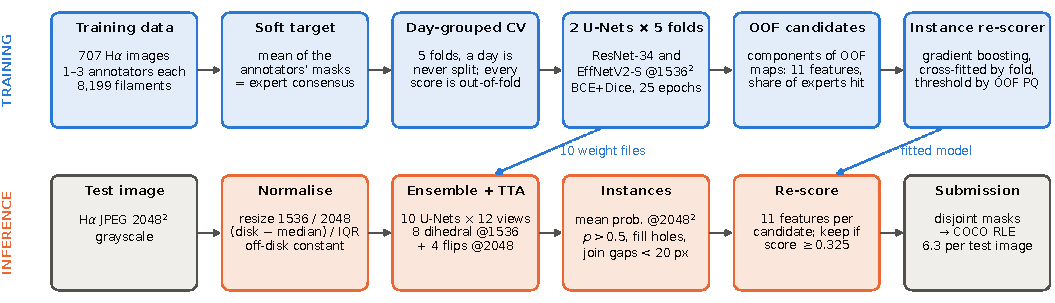
\includegraphics[width=\textwidth]{fig_pipeline.pdf}
  \caption{Pipeline. Training (top): soft consensus target, day-grouped 5-fold cross-validation, two U-Net encoders, and an
  instance re-scorer fitted on out-of-fold (OOF) candidates. Inference (bottom): disk standardisation, 10 models $\times$ 12
  views averaged at $2048^2$, connected components with fragment grouping, re-scoring, run-length encoding.}
  \Description{Two rows of boxes: a training lane and an inference lane, with arrows from trained weights and the fitted
  re-scorer to the inference steps that use them.}
  \label{fig:pipeline}
\end{figure*}

Figure~\ref{fig:pipeline} shows the whole pipeline; this section follows it from the data to the submitted masks.

\paragraph{Data, splits and validation.} The training set has 707 images, 1{,}154 annotator-images and 8{,}199 annotated
filaments, which cover only 0.36\% of the pixels. The images come from six GONG sites (Big Bear, Cerro Tololo, Learmonth,
Mauna Loa, El Teide and Udaipur). Frames of one day are near-duplicates, and 33 of the 180 test images share a day with a
training image, so we split the 656 observation days into five folds (137--148 images each): a day never straddles folds.
Every number below is out-of-fold (OOF) over all 707 images unless marked otherwise. We re-implemented the organisers' PQ
and unit-test it against a literal port of their self-evaluation notebook (identical TP, FP, FN and PQ). Uncertainty is a
95\% bootstrap interval over images~\cite{efron1993bootstrap} (2{,}000 resamples); differences between variants use a
paired bootstrap on the same images. The public leaderboard (LB) was only used to check predictions written down before
each submission, never to tune.
% src: run logs (fg frac 0.00356); configs/folds.csv (656 days; folds 137/137/142/143/148); ESTADO §4 (33 test images).

\paragraph{Pre-processing.} Each JPEG is read as grayscale and resized with area interpolation. Pixels of the solar disk
(grey level $>20$) are standardised with their median and IQR/1.349, clipped to $\pm8$ and divided by 4; off-disk pixels
get the minimum value. This removes most brightness and contrast differences between sites: OOF PQ varies only from
0.425 to 0.442 across sites (Fig.~\ref{fig:dist}d), so no site-specific step was needed.

\paragraph{Target.} Each annotator's polygons are rasterised with \texttt{pycoco\-tools}~\cite{lin2014coco} at $2048^2$ and
merged; the masks of the image's annotators are then averaged. The network thus learns a soft label (1/3, 1/2, 2/3 or 1
where experts agree partially or fully) instead of one expert's style.

\paragraph{Networks and training.} U-Nets~\cite{ronneberger2015unet} from \texttt{segmentation\_\allowbreak{}models\_\allowbreak{}pytorch}%
~\cite{iakubovskii2019smp} with ImageNet-pretrained~\cite{deng2009imagenet} encoders and one input channel: ResNet-34%
~\cite{he2016resnet} and EfficientNetV2-S~\cite{tan2021efficientnetv2,wightman2019timm}, both at $1536^2$. A U-Net is an
encoder--decoder: the decoder upsamples the encoder's coarse features and concatenates, through skip connections, the
encoder features of every scale, which keeps the thin, elongated boundaries that the IoU of PQ rewards. The two encoders
(residual blocks vs.\ MBConv and Fused-MBConv inverted bottlenecks) make different errors, so their average is better
than either (Table~\ref{tab:ablation}). The loss is BCE
plus soft Dice~\cite{milletari2016vnet} on the soft target; AdamW~\cite{loshchilov2019adamw} (learning rate $5\cdot10^{-4}$,
weight decay $10^{-4}$), one warm-up epoch and cosine decay, 25 epochs, batch 4, mixed precision on Kaggle's two T4 GPUs.
Augmentation runs on the GPU: flips and $90^\circ$ rotations, rotation $\pm15^\circ$, scale $\pm10\%$, contrast $\pm20\%$,
brightness and Gaussian noise. Each epoch visits every training image of the fold once, as a full image (no crops or
re-sampling), and the last-epoch weights are kept (no early stopping), so the validation fold never influences its model.
One model per fold and encoder gives 10 models (61 and 41 minutes per fold for EfficientNetV2-S and ResNet-34).
% src: kaggle/used_runs/run_*_1536.py; runs/*_1536_f0/log.txt (147 s and 98 s per epoch).

\paragraph{Inference.} Each model sees 12 views of the test image: the 8 dihedral transforms (flips of the image and of
its transpose) at $1536^2$ and the 4 flips at the native $2048^2$, where filaments look 33\% larger than in training. Every
map is transformed back, rounded to 1/255 (as the stored OOF maps used for tuning), resized bilinearly to $2048^2$ and
averaged with equal weight over the $10\times12$ maps.

\paragraph{Instances.} Pixels with $p\ge0.5$ are kept and holes are filled (annotated polygons are simple). The 8-connected
components of this mask \emph{dilated} by a disk of radius 10\,px define the instances, but only the original pixels are
kept: fragments up to about 20\,px apart become one filament without changing its shape. This addresses the
\emph{structural continuity} problem of filaments that break into several dark segments. Instances are disjoint by
construction, as the format requires.

\paragraph{Instance re-scoring.} Each candidate gets 11 features: log area; mean, maximum and 90th-percentile probability;
share of pixels with $p\ge0.7$; log total probability; bounding-box fill; elongation; boundary-to-area ratio; distance to
the disk centre; and number of candidates in the image. The target is the fraction of the image's annotators for which
the candidate is a TP. A histogram gradient-boosting regressor~\cite{pedregosa2011sklearn,ke2017lightgbm} (300 iterations,
learning rate 0.05, 15 leaves, $\ge40$ samples per leaf) is \emph{cross-fitted}: each fold's candidates are scored by a
model fitted on the other four folds. Candidates scoring $\ge0.325$, the threshold with the best OOF PQ, are kept. The
released re-scorer is refitted on all OOF candidates of the final ensemble. Choosing each fold's threshold on the other
four folds (nested) gives the same OOF PQ, 0.432, so the threshold choice is not optimistic.
% src: src/filseg/rescore.py, tools/rescore_fit.py (PARAMS); ablation.json row "FINAL..." nested_PQ 0.4318.

%%%%%%%%%%%%%%%%%%%%%%%%%%%%%%%%%%%%%%%%
%              EVALUATION              %
%%%%%%%%%%%%%%%%%%%%%%%%%%%%%%%%%%%%%%%%
\section{Evaluation}\label{sec:evaluation}
\paragraph{Overall.} The final model reaches OOF PQ \textbf{0.432} (95\% CI 0.423--0.441) with SQ 0.676 and RQ 0.639
(4{,}961 TP, 2{,}366 FP, 3{,}238 FN; 6.3 predictions per image). On the 296 multi-annotator images it scores 0.433, against
0.340 for one expert scored against the others. Per site it ranges from 0.425 (Cerro Tololo) to 0.442 (Udaipur), with
overlapping intervals (Fig.~\ref{fig:dist}d).
% src: stats.json: PQ 0.4318, SQ 0.6757, RQ 0.6391, TP/FP/FN 4961/2366/3238, pred_per_image 6.33,
%      PQ_multi_annotator_images 0.4334, per_site.

\begin{table}[t]
  \caption{Ablations, OOF PQ on 707 images (\dag: fold 0 only, 137 images, fixed rule). $\Delta$: paired difference to
  the block's reference or to the variant named in the row, with its 95\% bootstrap interval. E = EfficientNetV2-S,
  R = ResNet-34; *: compared with E + R with 4 flips (.427).}
  \label{tab:ablation}
  \footnotesize
  \setlength{\tabcolsep}{2.5pt}
  \begin{tabularx}{\columnwidth}{@{}Xcr@{}}
    \toprule
    Variant & PQ & $\Delta$ [95\% CI] \\
    \midrule
    \multicolumn{3}{@{}l}{\emph{Resolution and encoders} (4 flips, re-scorer)} \\
    R 1024 $\rightarrow$ R 1536 (grouping 12\,px) & .412 & $+.007$ [$+.002$, $+.012$] \\
    R on 1024 crops of $2048^2$ vs R 1536\dag & .404 & $-.007$ [$-.016$, $+.002$] \\
    E 1536 (reference) & .422 & -- \\
    E + R, both 1536 & .427 & $+.004$ [$+.000$, $+.008$] \\
    E + R + R 1024 vs E + R & .422 & $-.004$ [$-.007$, $-.002$] \\
    \midrule
    \multicolumn{3}{@{}l}{\emph{Test-time views} (E + R; reference: 4 flips at 1536)} \\
    8 dihedral views at 1536 & .428 & $+.002$ [$-.001$, $+.004$] \\
    4 flips at 2048 & .430 & $+.003$ [$-.002$, $+.008$] \\
    4 flips at 1536 + 4 at 2048 & .431 & $+.005$ [$+.001$, $+.008$] \\
    \textbf{8 at 1536 + 4 at 2048 (final)} & \textbf{.432} & $+.005$ [$+.002$, $+.008$] \\
    final + flips at 1792, 2304 vs final & .433 & $+.001$ [$-.002$, $+.004$] \\
    E fine-tuned at 2048 vs E\dag & .424 & $+.004$ [$-.007$, $+.015$] \\
    E + flips at 2048 vs E\dag & .434 & $+.014$ [$+.007$, $+.021$] \\
    \midrule
    \multicolumn{3}{@{}l}{\emph{Instance stage} (reference: final)} \\
    keep every candidate & .372 & $-.060$ [$-.064$, $-.056$] \\
    fixed rule (area $\ge$500, peak $\ge$0.9) & .418 & $-.014$ [$-.017$, $-.010$] \\
    pixel threshold 0.45 & .429 & $-.003$ [$-.005$, $-.001$] \\
    pixel threshold 0.55 & .431 & $-.000$ [$-.003$, $+.002$] \\
    no fragment grouping* & .420 & $-.007$ [$-.012$, $-.002$] \\
    grouping 6, 8 or 12\,px, not 10* & .426--.427 & within $\pm.001$ \\
    masks dilated by 1\,px* & .399 & $-.027$ [$-.032$, $-.023$] \\
    \midrule
    one expert vs.\ the others (296 img.) & .340 & [.325, .356] \\
    \bottomrule
  \end{tabularx}
\end{table}
% src: ablation.json (rows and vs_ref). Rows marked "4 flips" in the instance block are compared with E+R 4 flips g10 (0.4266).

\paragraph{Ablations (Table~\ref{tab:ablation}).} \emph{Resolution} helps: ResNet-34 gains $+0.007$ from 1024 to 1536\,px.
Training at the native 2048\,px on 1024 crops did not help ($-0.007$ on fold 0), and fine-tuning the 1536 models at 2048 gained only $+0.004$
(not significant), whereas simply adding 2048\,px views at test time gained $+0.014$ on the same fold. Multi-scale TTA
thus recovers the benefit of resolution at no training cost. A \emph{second encoder} adds $+0.004$, and a lower-resolution
third member hurts. The final 12-view TTA adds $+0.005$, and more scales add nothing measurable. The \emph{instance stage}
matters most: keeping every candidate costs $0.060$, and the best fixed rule instead of the re-scorer costs $0.014$.
Grouping fragments adds $0.007$ and is flat for radii of 6--12\,px, as is the pixel threshold between 0.5 and 0.55.
Dilating every mask by one pixel costs $0.027$: PQ is very sensitive to where the boundary lies.

\begin{figure*}[t]
  \centering
  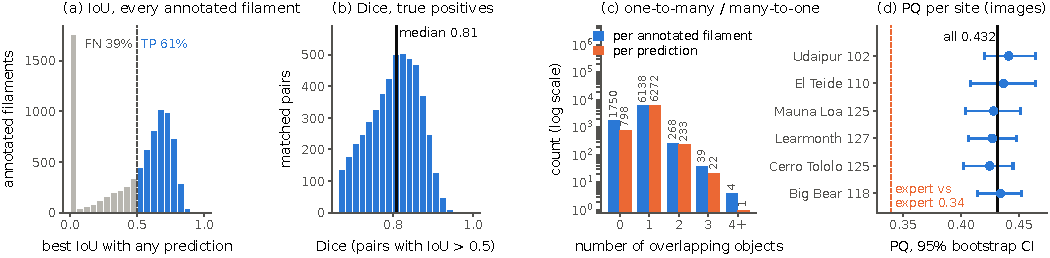
\includegraphics[width=\textwidth]{fig_distributions.pdf}
  \caption{Final model, OOF on 707 images. (a) Best IoU of each of the 8{,}199 annotated filaments with any prediction
  (TP if $>0.5$). (b) Dice of the 4{,}961 matched pairs. (c) One-to-many (an annotated filament touched by several
  predictions) and many-to-one counts. (d) PQ per GONG site with 95\% bootstrap intervals; dashed: one expert against
  the others.}
  \Description{Four panels: an IoU histogram with a large bar at zero and a peak near 0.7, a Dice histogram peaking near
  0.82, log-scale bar counts of overlaps, and per-site PQ dots with error bars between 0.40 and 0.47.}
  \label{fig:dist}
\end{figure*}

\paragraph{Distributions (Fig.~\ref{fig:dist}).} Matched pairs have mean IoU 0.676 and mean Dice 0.803 (medians 0.68 and
0.81). Of the 8{,}199 annotated filaments, 61\% are matched, 12\% are near misses (best IoU 0.3--0.5, median area
1{,}675\,px, mostly disagreements on the extent of large filaments) and 21\% are not touched by any prediction. Size is the
main factor: recall is 0.36 below 500\,px and 0.65--0.69 above 1{,}000\,px, and half of the missed filaments are smaller
than 1{,}000\,px. Fragmentation and merging are rare: 311 annotated filaments (3.8\%) are touched by two or more
predictions, and 256 predictions (3.5\%) touch two or more annotated filaments.
% src: stats.json (tp_iou_mean 0.6757, tp_dice_mean 0.8034, medians, annotated_* counts, overlap counts);
%      runs/fn_size_s10.log (recall by area, 51.6% of FN < 1000 px, near-miss median area 1675).

\begin{figure}[t]
  \centering
  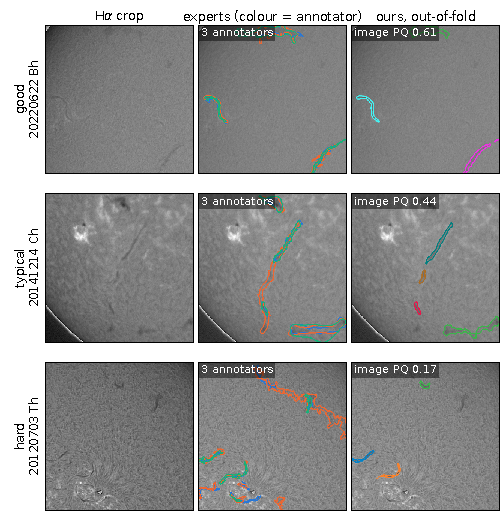
\includegraphics[width=\columnwidth]{fig_examples.pdf}
  \caption{Out-of-fold examples ($560\times560$\,px crops of the $2048^2$ images). Good: all three experts' filaments found with
  smooth, single-piece masks. Typical: a long filament that one expert draws as a single object is split into three
  pieces. Hard: dense small filaments near an active region and a long faint channel are mostly missed.}
  \Description{Three rows of image crops: raw H-alpha, experts' outlines in one colour per annotator, and our outlines in
  one colour per predicted filament.}
  \label{fig:examples}
\end{figure}

\paragraph{Morphology (Fig.~\ref{fig:examples}).} Predicted masks are smooth, single-piece and follow the dark core of the
filament, so they agree with all experts where the experts agree with each other. Thin barbs and the faint ends that only
some experts include are usually left out, which lowers the IoU of large filaments. Long, faint filaments can split into
pieces when their middle falls below the threshold, and crowded active regions remain the hardest case.

\begin{table}[t]
  \caption{Validation vs.\ public leaderboard for the submissions with full OOF estimates, sorted by OOF PQ. PQ$'$:
  expected score if test experts drew a fraction $r=0.736$ of the filaments (Eq.~\ref{eq:pqprime}).}
  \label{tab:lb}
  \footnotesize
  \setlength{\tabcolsep}{3pt}
  \begin{tabularx}{\columnwidth}{@{}lXccc@{}}
    \toprule
    & Model and selection & OOF PQ & PQ$'$ & LB \\
    \midrule
    s03 & R 1024 $\times$5, fixed rule & .390 & .332 & .33 \\
    s04 & s03 + re-scorer & .400 & .343 & .34 \\
    s07 & E + R 1536, fixed rule & .416 & .357 & .35 \\
    s08 & E + R, strict re-scorer (0.45) & .421 & .363 & .36 \\
    s06 & E + R, re-scorer & .427 & .366 & .37 \\
    s09 & s06 + 4 flips at 2048 & .431 & .370 & .37 \\
    s10 & s06 + 8 views at 1536, 4 at 2048 (final) & .432 & .369 & .38 \\
    \bottomrule
  \end{tabularx}
\end{table}
% src: ablation.json "submissions" (oof_PQ, PQ_prime_fit with r_least_squares 0.736); LB from ESTADO §5.

\paragraph{Validation vs.\ leaderboard (Table~\ref{tab:lb}).} The LB is lower than OOF (LB/OOF 0.84--0.88) but ranks our
seven fully validated submissions in the same order (Spearman 0.99, Pearson 0.98): no pair of them is ordered
differently by OOF and LB (s06 and s09 tie at 0.37). Our model behaves alike on both sets (6.27 predicted filaments per test
image vs.\ 6.33 OOF), so we attribute the gap to the test annotations. If a test expert draws only a fraction $r$ of the
filaments a training expert would draw, a fraction $1-r$ of our TPs become FPs and the FNs shrink by $r$:
\begin{equation}
  \mathrm{PQ}'=\frac{r\,\Sigma}{r\,\mathrm{TP}+\frac12\mathrm{FP}+\frac12(1-r)\,\mathrm{TP}+\frac12 r\,\mathrm{FN}},
  \label{eq:pqprime}
\end{equation}
with $\Sigma$ the summed IoU of the TPs. With one least-squares $r=0.736$, PQ$'$ reproduces all seven LB scores within 0.011,
against a display precision of $\pm0.005$. The public LB uses about 90 images, so its own sampling error is about
$\pm0.03$; paired differences between submissions are far more precise than that. We cannot verify $r$ without the
test labels, which we did not use (the full MAGFiLO release contains them).
% src: ablation.json summary: lb_over_oof_range_full [0.842, 0.880], spearman 0.991, pearson 0.975, r_least_squares 0.736,
%      max_abs_residual_at_r_fit 0.0107; test filaments: s10 CSV 1,129 rows / 180 images = 6.27.
%      ±0.03: OOF CI half-width 0.009 on 707 images scaled by sqrt(707/90) ≈ 2.8 (approximation, stated as "about").

\paragraph{Strengths, weaknesses and improvements.} \emph{Strengths:} the consensus target and the re-scorer optimise what
PQ rewards; no hand-tuned image processing; stable across the six sites; disjoint masks with few fragments or merges; and
a validation protocol that predicted the LB. \emph{Weaknesses:} small filaments ($<1{,}000$\,px) account for half of the
misses; barbs and faint filament ends are smoothed away; long faint filaments can break into pieces; and inference is
heavy (120 network passes, 17.8\,s per image on a T4). \emph{Improvements:} training at native resolution with more
memory; using the filament spines that MAGFiLO provides as an auxiliary training target; a boundary-refinement step
for barbs; and learning the fragment grouping instead of using a fixed radius.

\paragraph{Reproducibility.} The repository holds the package \texttt{src/filseg} (data, model, post-processing,
re-scorer, metric and pipeline modules), the training scripts that produced the released models, the 10 weight files
(45--49\,MB each), the fitted re-scorer, \texttt{requirements.txt} with exact versions, and a notebook that runs the whole
inference pipeline from \texttt{configs/\allowbreak{}final\_all.json}. Scripts in \texttt{tools/} regenerate every table and figure of
this report from the OOF maps. We checked the notebook in a clean Kaggle kernel: a fresh virtual environment with exactly
\texttt{requirements.txt} (Python 3.13, PyTorch 2.15, Tesla T4) ran it end to end on every fifth test image (36 images).
It gave the same number of filaments as our submitted file on every image (201 in total), and every filament matched its
submitted mask with IoU $\ge0.998$; 176 masks were bit-identical, and the rest differ by boundary pixels from fp16
arithmetic. Inference takes 17.8\,s per image on a T4, about 53 minutes for the 180 test images. Training the 10
released models took 9.4 GPU-hours of Kaggle sessions, and all experiments together about 19.
% src: clean check run_summary.json / compare.json (36 images, 201 = 201, matched_iou_min 0.9979, identical_rle 176,
%      notebook cell 3: 640.9 s / 36 images = 17.8 s); weights/ file sizes 44.8 MB and 49.0 MB;
%      GPU hours: ESTADO §6 (EffV2S-1536 1.14+2.2+2.25, R34-1536 0.8+1.5+1.5 = 9.4 h; total ≈ 19.3 h on 11-nov).

%%%%%%%%%%%%%%%%%%%%%%%%%%%%%%%%%%%%%%%%
%            ACKNOWLEDGMENT            %
%%%%%%%%%%%%%%%%%%%%%%%%%%%%%%%%%%%%%%%%
\section{Acknowledgment}\label{sec:acknowledgment}
    % Do not change
    The organization of the Filament Segmentation Challenge 2026 is partially supported by the U.S. National Science Foundation (NSF) under Grant No. 2209912 and 2433781, directorate for Computer and Information Science and Engineering (CSE), and Office of Advanced Cyberinfrastructure (OAC), and Grant No. 2511630, AST Division Of Astronomical Sciences and MPS Directorate for Mathematical and Physical Sciences.

    The Filament Segmentation Challenge 2026 is sponsored by the U.S. National Science Foundation (NSF) National Solar Observatory (NSO).

    This work utilizes GONG data obtained by the NSO Integrated Synoptic Program, managed by the National Solar Observatory, which is operated by the Association of Universities for Research in Astronomy (AURA), Inc. under a cooperative agreement with the National Science Foundation and with contribution from the National Oceanic and Atmospheric Administration. The GONG network of instruments is hosted by the Big Bear Solar Observatory, High Altitude Observatory, Learmonth Solar Observatory, Udaipur Solar Observatory, Instituto de Astrofísica de Canarias, and Cerro Tololo Interamerican Observatory.

\bibliographystyle{ACM-Reference-Format}
\bibliography{main}

\end{document}
